\documentclass[12pt]{article} 
\usepackage[left=2cm, right=2cm, top=2cm, bottom= 2cm]{geometry} 
\usepackage{graphicx,epsfig,verbatim,enumerate}
\usepackage{amssymb,amsmath,amsthm,amsbsy}
\usepackage{ifthen}
\usepackage{morefloats}
\usepackage[hidelinks]{hyperref}
%\hypersetup{colorlinks=true, linkcolor=blue}
\usepackage{cite}
\usepackage{color}
\usepackage{textcomp}
\usepackage{float}
\usepackage{subfig}

\newcommand{\todo}[1]{\noindent\textcolor{blue}{{$\Box$ #1}}}

\title{Mixed and Pure Breed Dog Classifier}
\date{\today}
\author{Luke Trinity and Nat Shenton \\ CS 254}

\begin{document} 
\maketitle
\section{Introduction}

Online sources of high resolution images including Google, Image-net \cite{deng2009imagenet}, and Flickr are providing new opportunities to explore applications of image categorization using computer vision. One interesting application in the field of fine-grained image classification is identification of dog breed. Dogs are considered to be highly differentiable for each breed, which makes classification an approachable problem. However, the work is challenging due to the varying combinations of facial characteristics and color patterns between species, as well as intra-class variation within a single species. Another aspect of the problem that makes it more complicated is the presence of humans and man-made backgrounds, which are not as common in other animal datasets. Many machine learning algorithms exist to classify pure-bred dogs, but none are currently available to identify mixed breed dogs. To address this gap in available tools, we aimed to build a classifier that identifies dogs as mixed or pure-bred. Our approach will be to test multiple types and configurations of models on an existing pure-bred dog image classification dataset \cite{khosla2011novel}, in combination with a mixed breed dataset we built ourselves using paired DNA test results and photos \cite{voith2009comparison} as well as crowd sourced mixed breed dog images. 

\section{Problem Definition and Algorithm}

\subsection{Task Definition}

The task is to take dog images where each image is labeled either mixed or pure-bred and use them to train an algorithm to classify an unseen photo based on whether the dog is mixed or pure. An important part of training our neural network is to normalize the input images. Each input image is defined as a matrix of $224\times 224\times3$. The output of this algorithm will either be a mixed or pure-bred dog. Potential benefits of this work are to provide dog owners an easy way to classify if their dog is a pure-bred or mixed, in addition to assisting shelters in generating interest in dogs to increase adoption rates. From a machine learning perspective, our testing suite produces interesting and thought-provoking results about how to select and configure a model in a difficult decision space. It could be an exciting way to start a conversation and help people learn about different breeds of dogs, and how they are mixed. The final goal for this task would allow for a dog owner to upload a picture of their dog to a website or app, and have the classifier identify their dog as mixed or pure-bred.

\subsection{Dataset}

The Stanford Dogs Dataset has 20,580 images, with 120 total classes of dog breed. \cite{khosla2011novel} Each image also has an associated bounding box identifying the location of the dog within the photo. The mixed-breed dataset from Voith et al. \cite{voith2009comparison} has 20 images each paired with DNA percentage breakdown of dog breed. We used crowdsourcing to generate 246 additional mixed breed dog pictures. One assumption of our dataset was that when we asked for friends to submit photos of their mixed breed dogs, we assume that they are in fact mixed breed. There was no way to identify if the dog was actually mixed without DNA testing. The final balanced dataset was obtained by taking a random sampling of pure-bred dogs from the Standard dataset equal to the number of images in the mixed breed dataset, giving 532 total images (266 pure-bred, 266 mixed breed). 

\subsection{Algorithm Definition}

First, we utilize the Resnet50 convolutional neural network \cite{he2015deep} as it achieves roughly 80\% accuracy on the Stanford dog dataset in classifying pure-bred dogs. This pretrained neural network gives a classification accuracy high enough that it will classify an image of a pure-bred dog correctly most of the time. The Resnet50 convolutional neural network is trained on Google's ImageNet which contains the Stanford Dogs dataset. The CNN takes an image as an input, and outputs a vector of probabilities with labels identifying dog breed. Our algorithm took the four highest probabilities in the vector and then implemented principal component analysis to take the four prediction outputs down to two features. For each of the 532 images and their associated two features, we used cross validation to test four different classification methods: linear kernel SVM, optimal kernel SVM, random forest, and neural network. Due to the limited size of our dataset, the random split of testing and training data results in variation in model performance. To account for this we average over 250 different split of the testing and training data, as described in the experimental methods section.

\begin{figure}[H]
\centering{
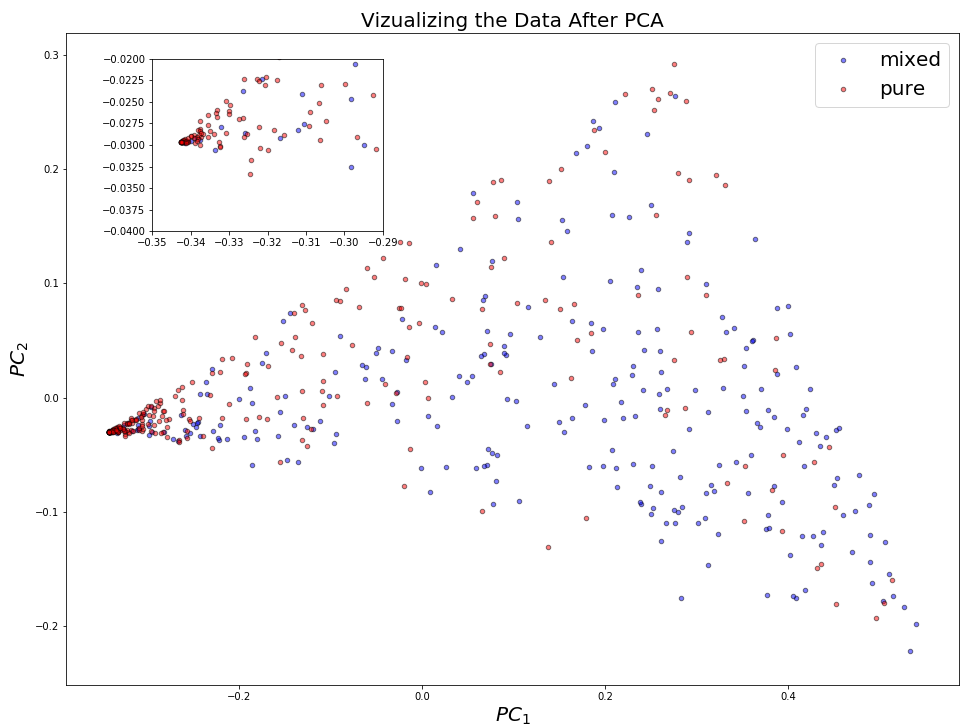
\includegraphics[width=0.55\textwidth]{Data_vis}
}
\caption{The distribution of the data after using principal component analysis to reduce the breed probabilities from a vector of length four to only two features. Red is pure-bred while blue is mixed. The inset plot shows the area where the data is clustered.}
\end{figure}

\section{Experimental Evaluation}

\subsection{Methodology}

For the SVM linear kernel we used cross-validation to search over C values randomly drawn from an exponential distribution (scale=1000), $\gamma$ values were randomly drawn from an exponential distribution (scale = 2), and we also validate over balanced or no class weight. For the SVM optimal kernel, the cross-validation searches over Radial Basis Function kernel and polynomial kernel. The random forest algorithm looks at a forest of 30 trees, and draws randomly from a uniform distribution for the minimum number of samples to split on as a fraction of the total number of samples. For random forest we also validated for max depth by randomly choosing an integer between 1 and 50. Before moving on to the description of neural network testing, please note that for the cross validation specified above 15 fold was used across model types. In addition, the randomized search cross validation iterated 200 times for each model.

\begin{figure}[H]
\centering{
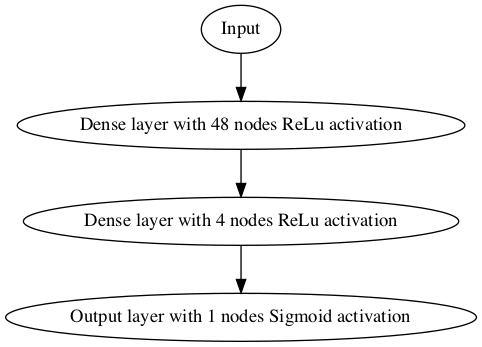
\includegraphics[width=0.6\textwidth]{nueral_netgv}
}
\caption{Neural Network Structure}
\end{figure}

The neural network uses an architecture of 3 hidden fully connected layers with the ReLu activation function. The first layer contains 48 neurons, the second 24 neurons, and the third 4 neurons; each with bias and kernel constraints. The output layer contains one neuron with a sigmoid activation function. The model was compiled with the Adam gradient descent optimizer, and binary cross-entropy as the loss function. The neural network was trained over 300 epochs. 

For each of the four model types described, we trained as outlined above, and tested 250 different splits of the data with a 66-33 training testing split. Here we report the accuracy, as well as the difference between the training and test accuracy, for each of those 1000 models grouped by model type.

\begin{figure}[H]
\centering{
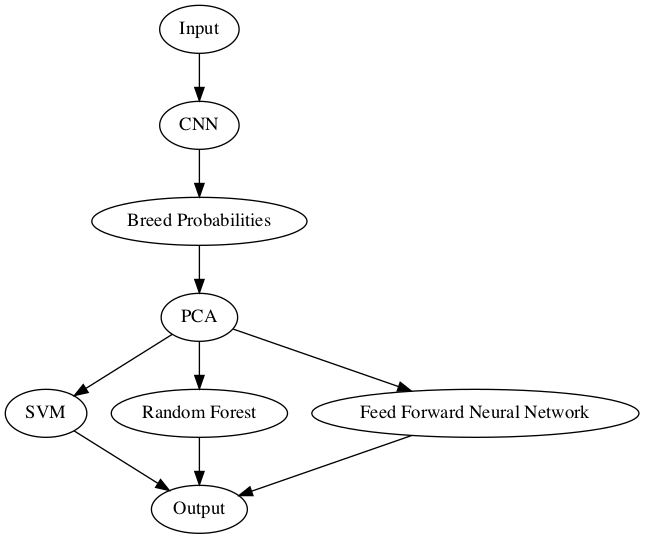
\includegraphics[width=0.6\textwidth]{modelgv}
}
\caption{Model Testing Suite Visualization}
\end{figure}

\subsection{Additional Neural Network Methodology}

In the results section we present the conclusion that neural networks are performing the best on our dataset. To further test how different neural network architectures might affect accuracy, we increased and decreased the number of neurons in our hidden layers and ran a similar experiment to the one described above. This second testing suite is used to compare three different neural network architectures. In addition to our initial neural network (48, 24, and 4 neurons in each hidden layer) which we will refer to as `medium’ depth, we also test a `less deep’ model (24, 12, and 2 neurons in each hidden layer) and a deeper model (96, 48, and 8 neurons in each hidden layer). The same bias and kernel constraints were used for each of the neural networks, which were trained for 300 epochs each on the same 250 splits of the data. We also used mini-batch of size 128, which lead to slightly improved performance of the `medium’ depth neural network (Table 1 vs. Table 3). For these 750 total models tested, we again report the accuracy and training-test accuracy distributions.

\section{Results}

\subsection{Comparing SVM, Random Forest, and Neural Network methods}

Here we present the results of the initial testing suite. Table 1 describes the mean and standard deviation of model accuracy on the test split by model type. SVM with linear kernel, SVM with a non-linear kernel, and random forests perform about the same. The neural network was identified as performing the best, with 78\% accuracy. 

\begin{table}[H]
\centering
\begin{tabular}{|l|c|c|}
\hline
\multicolumn{1}{|l|}{Model Type} & Mean & \multicolumn{1}{l|}{Standard Deviation} \\ \hline
SVM (linear kernel) & 0.747 & 0.026 \\
\hline
SVM (optimal kernel) & 0.753 & 0.024 \\
\hline
Random Forest & 0.742 & 0.030 \\
\hline
Multi Layer Perceptron & 0.780 & 0.028 \\
\hline
\end{tabular}
\caption{Mean and standard deviation of model accuracy for 250 different splits of the dataset.}
\end{table}

Figure 4 displays the distribution of accuracy scores for each model type. Here we demonstrate that in addition to having the highest mean accuracy, the neural network also has the highest maximum and minimum. This can be interpreted as indicating the neural network has the most potential to be the best classifier, and also that even if it is not performing well, the worst-case scenario is relatively better than other model types (SVM or Random Forest).

\begin{figure}[H]
\centering
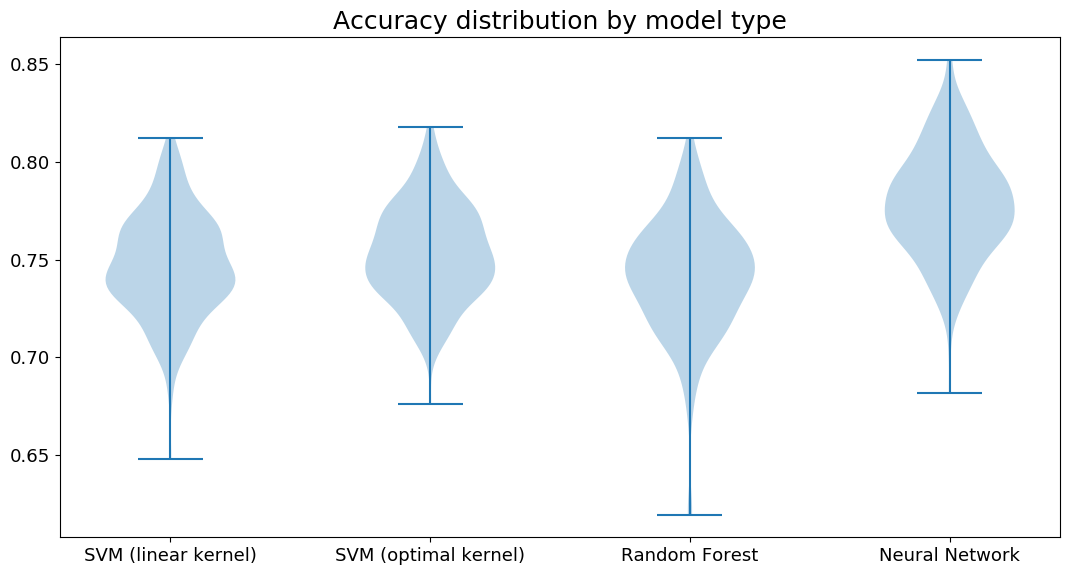
\includegraphics[width=0.7\textwidth]{testOut}
\caption{Violin plot of model accuracy by classification method.}
\end{figure}

In addition to recording the accuracy of our models on the testing split, we were also interested in calculating a metric to identify overfitting. To accomplish this, we recorded the difference between the model accuracy on the training split vs. the testing split ($\text{Accuracy}_{\text{Testing}} - \text{Accuracy}_{\text{Training}}$). If overfitting is occurring, we can expect the model to do much worse on the testing split. In Table 2 we present the mean and standard deviation of these differences over the 250 testing splits; with a positive value indicating higher accuracy on the testing split than the training, and a negative value indicating lower accuracy on the testing split than the training. Here it can be seen that although the neural network is performing the best (Table 3, Figure 4), it is also overfitting the most. On average the neural network had an 8\% accuracy decrease from training to testing.

\begin{table}[H]
\centering
\begin{tabular}{|l|c|c|}
\hline
\multicolumn{1}{|l|}{Model Type} & Mean & \multicolumn{1}{l|}{Standard Deviation} \\ \hline
SVM (linear kernel) & -0.003 & 0.039 \\
\hline
SVM (optimal kernel) & -0.014 & 0.036 \\
\hline
Random Forest & -0.022 & 0.039 \\
\hline
Multi Layer Perceptron & -0.080 & 0.039 \\
\hline
\end{tabular}
\caption{ Mean and standard deviation of $\text{Accuracy}_{\text{Testing}} - \text{Accuracy}_{\text{Training}}$ for 250 different splits of the dataset by model type.}
\end{table}

Figure 5 presents the distribution of the $\text{Accuracy}_{\text{Testing}} - \text{Accuracy}_{\text{Training}}$ for each model. This gives a representation of the overfitting the models could be experiencing. Here it can be seen that the neural network has the greatest potential to overfit, while the linear kernel is not overfitting at all. 

\begin{figure}[H]
\centering
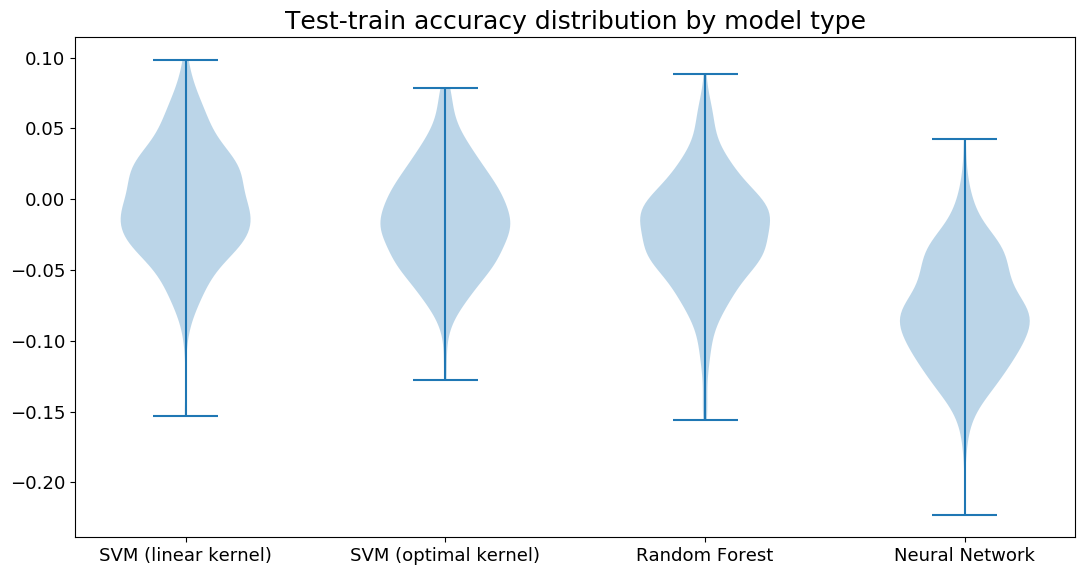
\includegraphics[width=0.7\textwidth]{testOut2}
\caption{ Violin plot of model $\text{Accuracy}_{\text{Testing}} - \text{Accuracy}_{\text{Training}}$ by classification method.}
\end{figure}

In Figure 6 we present a decision boundary produced by the neural network architecture described above. In the next section we will contrast this boundary with a different result, produced by a neural network with more neurons in each hidden layer. 

\begin{figure}[H]
\centering
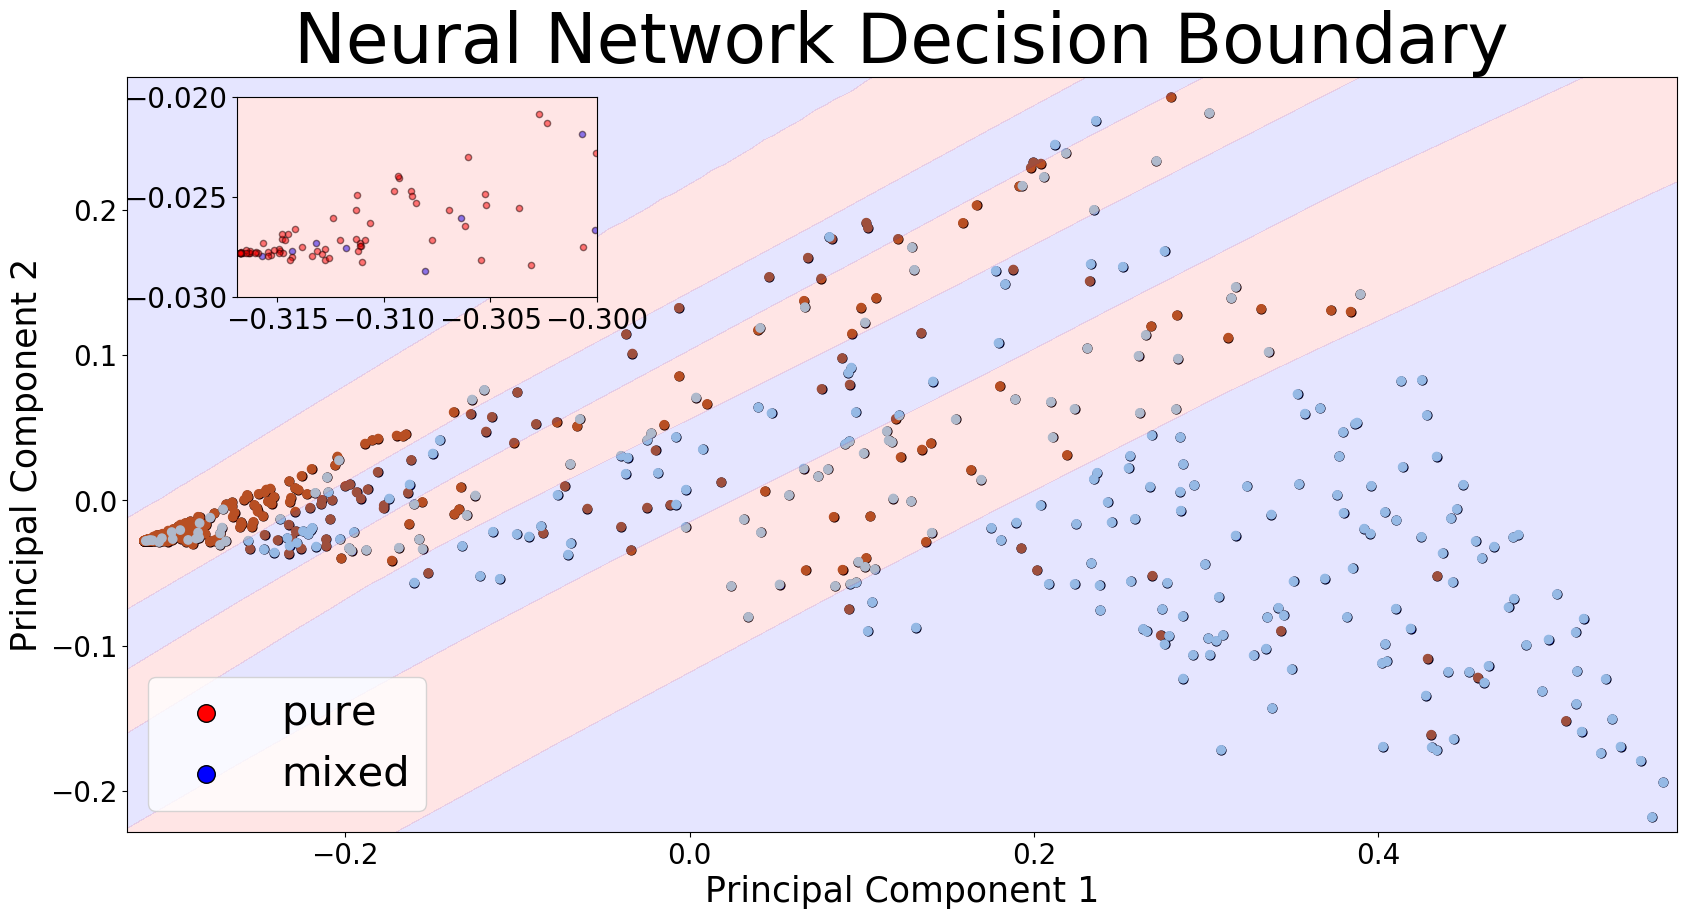
\includegraphics[width=0.6\textwidth]{initialboundary}
\caption{Example decision boundary of neural network.}
\end{figure}

\subsection{Comparing Neural Network Architectures}

After determining that the neural network was performing better than other models, we looked to vary the architecture of our multi-layer perceptron to potentially increase our accuracy. Building out from our initial medium depth neural network (48, 24, and 4 neurons in each hidden layer), we also tested a less deep model (24, 12, and 2 neurons in each hidden layer) and a deeper model (96, 48, and 8 neurons in each hidden layer). Here we present the results in Table 3, showing that we were able to increase our mean accuracy to 80\% with the deeper architecture. 

\begin{table}[H]
\centering
\begin{tabular}{|l|c|c|}
\hline
\multicolumn{1}{|l|}{Model Type} & Mean & \multicolumn{1}{l|}{Standard Deviation} \\ \hline
Least Deep (24-\textgreater{}12-\textgreater{}2-\textgreater{}1) & 0.7899 & 0.027 \\
\hline
Medium Depth (48-\textgreater{}24-\textgreater{}4-\textgreater{}1) & 0.7863 & 0.025 \\
\hline
Deepest (96-\textgreater{}48-\textgreater{}8-\textgreater{}1) & 0.7966 & 0.030 \\
\hline
\end{tabular}
\caption{Mean and standard deviation of model accuracy for 250 different splits of the dataset.}
\end{table}

Here we demonstrate the increased robustness of a deeper model in Figure 7. For the deepest architecture, in addition to a higher mean, we also have an increased minimum reported accuracy, and at least one of the deeper models achieved close to 90\% accuracy which was previously unseen. 

\begin{figure}[H]
\centering
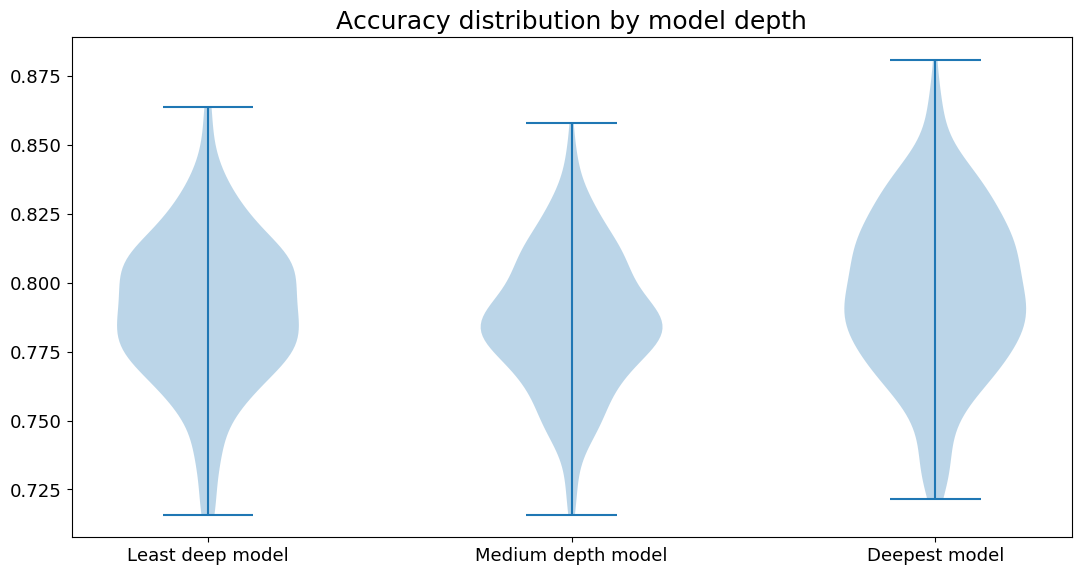
\includegraphics[width=0.7\textwidth]{testOut128}
\caption{ Violin plot of model accuracy by architecture.}
\end{figure}

While the deepest neural network is performing the best on average, here we present the results of the $\text{Accuracy}_{\text{Testing}} - \text{Accuracy}_{\text{Training}}$ for each architecture in Table 4 and Figure 8. As expected, when we increase the number of neurons in each hidden layer, we observe increased overfitting. 

\begin{table}[H]
\centering
\begin{tabular}{|l|c|c|}
\hline
\multicolumn{1}{|l|}{Model Type} & Mean & \multicolumn{1}{l|}{Standard Deviation} \\ \hline
Least Deep (24-\textgreater{}12-\textgreater{}2-\textgreater{}1) & -0.027 & 0.035 \\
\hline
Medium Depth (48-\textgreater{}24-\textgreater{}4-\textgreater{}1) & -0.055 & 0.037 \\
\hline
Deepest (96-\textgreater{}48-\textgreater{}8-\textgreater{}1) & -0.102 & 0.042 \\
\hline
\end{tabular}
\caption{ Mean and standard deviation of $\text{Accuracy}_{\text{Testing}} - \text{Accuracy}_{\text{Training}}$ for 250 different splits of the dataset by network architecture.}
\end{table}

\begin{figure}[H]
\centering
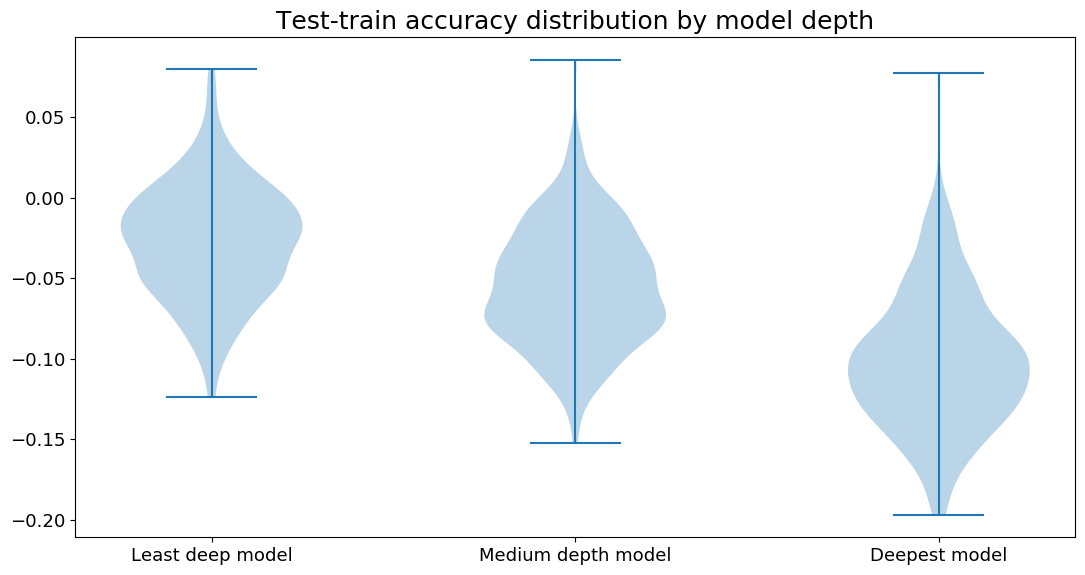
\includegraphics[width=0.7\textwidth]{testOut1289}
\caption{ Violin plot of model $\text{Accuracy}_{\text{Testing}} - \text{Accuracy}_{\text{Training}}$ by arc.}
\end{figure}

In Figure 9 below we visualize the decision boundary resulting from training one of our deepest neural networks. In comparison to Figure 6, the medium depth model, here we see increased flexibility in the classification output.

\begin{figure}[H]
\centering
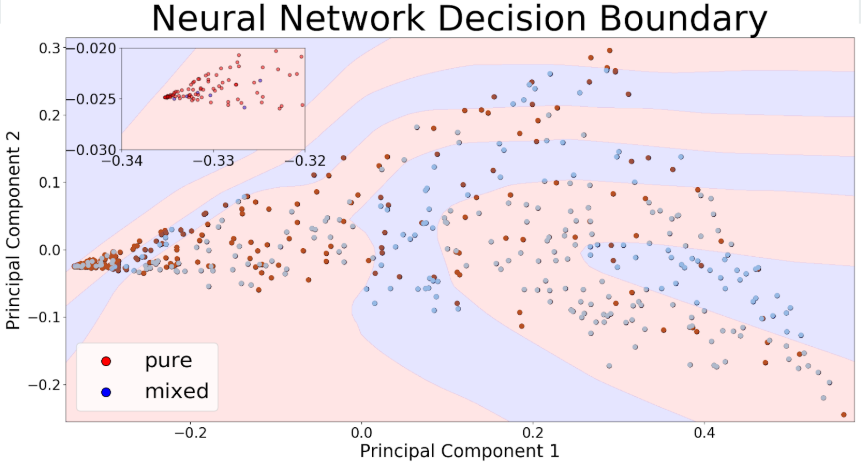
\includegraphics[width=0.6\textwidth]{updatedboundary}
\caption{Example decision boundary of deepest neural network.}
\end{figure}


\subsection{Discussion}

Our initial testing determined that neural networks were performing better than SVM or random forest, with a mean accuracy of 78\%. We continued our analysis by comparing three different architectures to determine if we could potentially further increase accuracy. Our deepest neural networks were averaging 80\% accuracy, which shows that we were successful. However, if we had more time, we would continue tuning hyperparameters in the hopes of further increasing our accuracy. This work is interesting and thought-provoking from a machine learning perspective, because of the way we implanted a testing suite to deal with variability when using a smaller dataset. Here we explored many concepts discussed over the semester, and present results that show we carefully thought through the work in the hopes of legitimately increasing our classification accuracy. 

Towards the end of the semester, we also worked to set up a demonstration for the CS Fair that could showcase our classifier. In order to do this, we set up a Flask web applet running in a Jupyter notebook on an Amazon Web Services server. The applet loaded both our own model as well as the Resnet50, and waited for a user to submit an image of a dog in the browser using an HTML form. When the user submitted the form, the applet received the image, and utilized our algorithm to classify the image as a mixed or pure-bred dog. Here we present screenshots of our demo in action, which was an excellent conversation starter and shows the scalability of this work. 

\begin{figure}[H]
\subfloat[][]{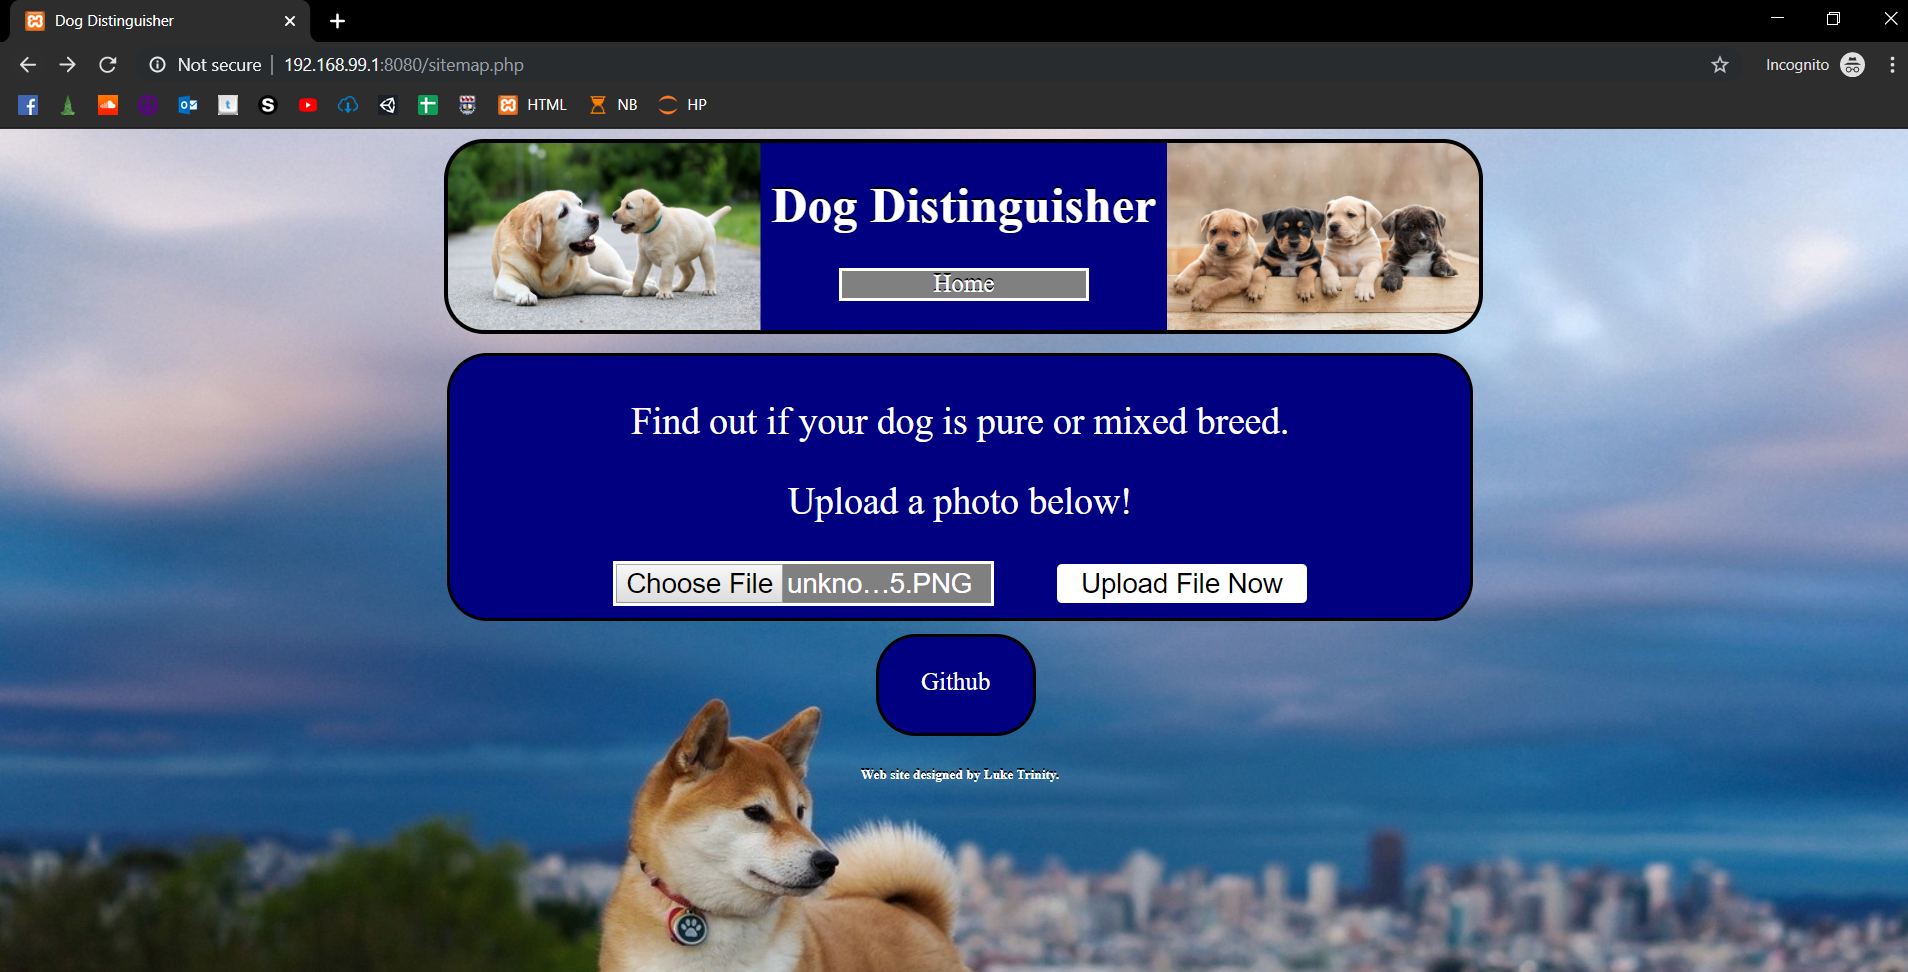
\includegraphics[width=23em]{screenshot1}}
\vspace{1cm}
\subfloat[][]{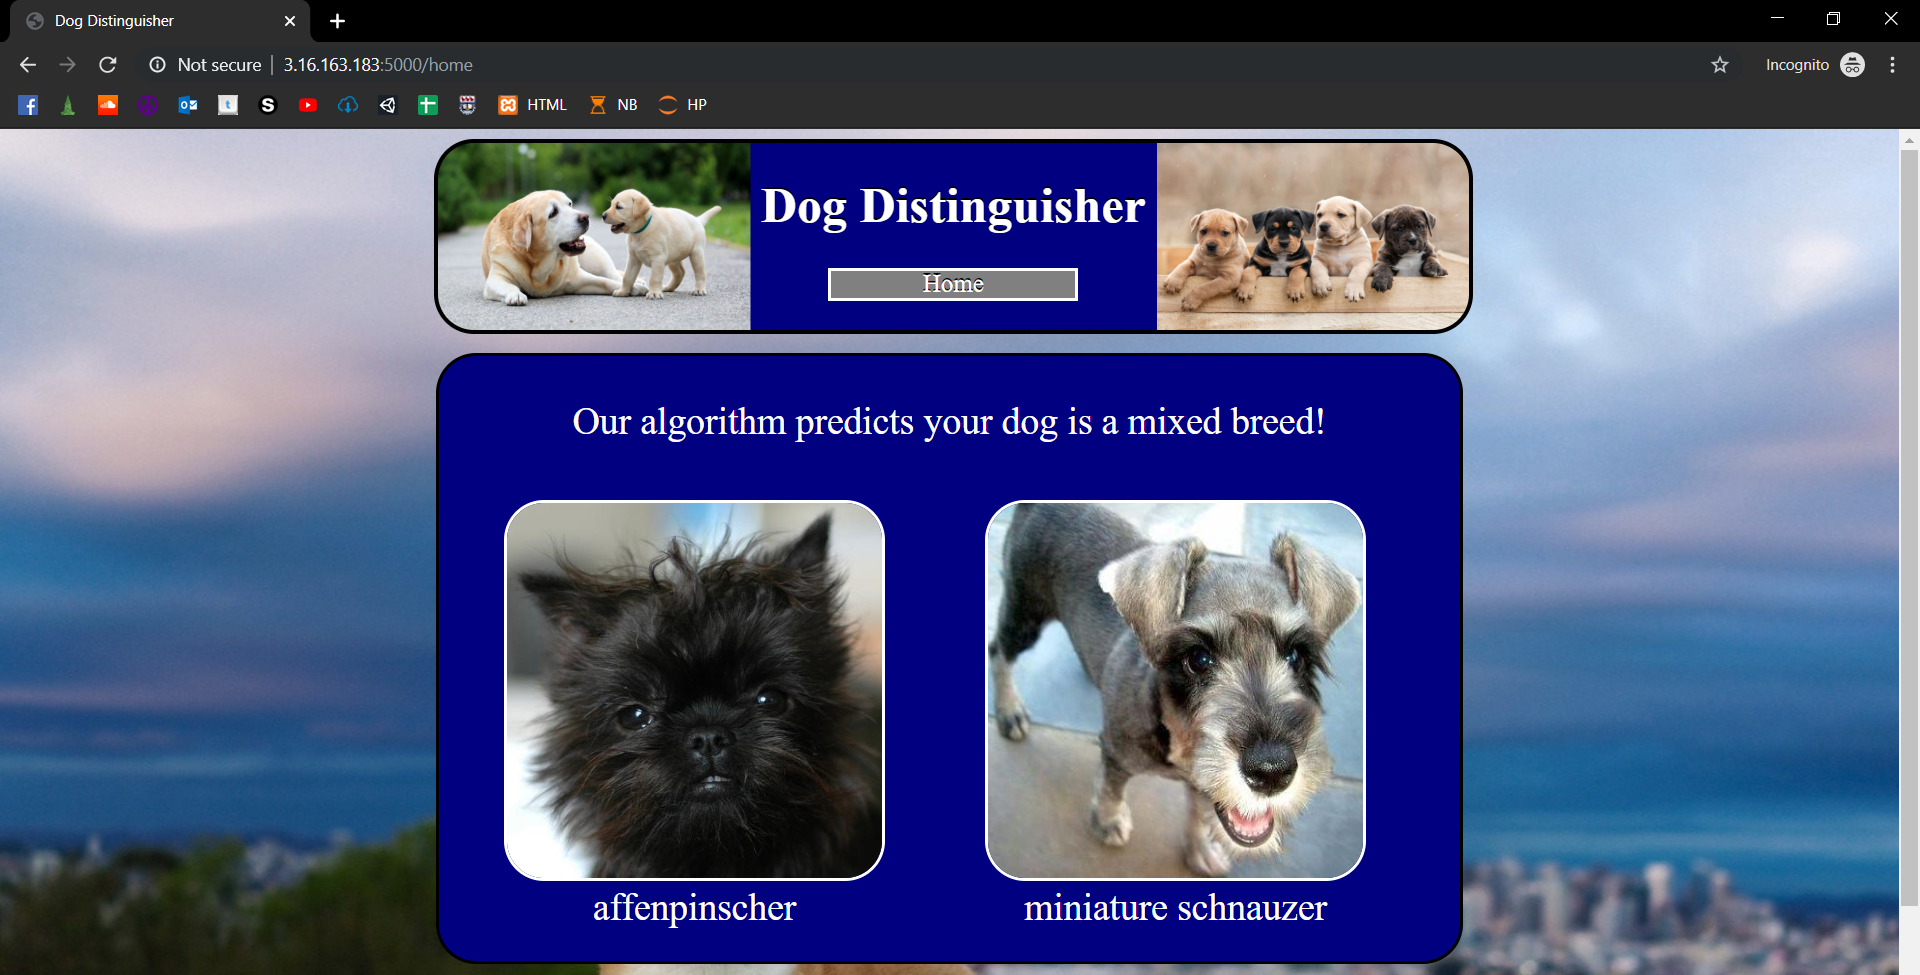
\includegraphics[width=23em]{screenshot2}}
\caption{Screenshots of user interface, (a) shows the html page where the user uploads an image using an HTML form, (b) shows the resulting output to the user after the Flask web applet running on Amazon Web Services returns the result from our classifier.}
\end{figure}


\section{Related Work}

In the initial article utilizing the novel dataset by Khosla et al. \cite{khosla2011novel}, the mean accuracy reached 22\% when 100 training images were utilized within the SIFT methodology. Liu et al. \cite{liu2012dog} reached 69\% accuracy, with greater success than Khosla et al. \cite{khosla2011novel} due to their partially localized approach. Several bounding box approaches are currently being reviewed, one is a slight adaptation to a method often employed for images of different shade and dimension called DeepCut. \cite{rajchl2016deepcut} There are several standard variations on the basic DeepCut methodology, which hone in on the nature and dimension of the bounding in a cookie-cutter, traced-out way as opposed to any kind of geometric shape. There was also a Kaggle competition to create the best dog breed classifier of 16 breeds sampled from the Stanford Dog dataset. Here competitors use transfer learning to create the best breed classifier. Competitors were able to get classification scores above 95\% in this competition \cite{kaggledogs}. Microsoft has a dog classifier built on their Bing platform, this platform was used as inspiration for our own web app.

\section{Code and Dataset}

The code can be found in our github repo: \url{https://github.com/nshenton/CS_251_DogProject}. Please see the Readme in the repo for more information. The Stanford Dogs Dataset can be downloaded from this page: \url{http://vision.stanford.edu/aditya86/ImageNetDogs/}. Please contact the authors for the mixed dog dataset.

\section{Conclusion}

Classifying dogs as pure or mixed breed is still a difficult problem as there is a great deal of diversity among all dogs and images taken of them. The dataset produced a great deal of variability based on the training and testing split because it was smaller. We worked to address this by building a testing suite to remove some of this variability. Here we have defined a methodology to test different models and configurations of machine learning. The neural network was identified as the best method to classify mixed dog breeds based on our method. Moreover, the deepest neural networks had slightly increased average accuracy than our initial network architecture. Obtaining 266 images of mixed breed dogs over the semester was a good first attempt at crowdsourcing labeled images using a social network. In the future, a larger dataset would be helpful in creating a more robust classifier. In addition, the hyperparameter of the first convolutional network (Resnet50) could be optimized by using transfer learning to achieve better results on the initial breed classification. Overall the project is a great conversation starter for dog lovers and machine learning enthusiasts alike, where an image can be classified as mixed or pure-bred in a scalable online platform. 

\nocite{*}
\bibliography{dogbib}{}
\bibliographystyle{ieeetr}

\end{document}


